\section{Proof of concept: hand-gesture solution}
\label{sec:hands}
This solution was developed to test that the flow of the application works as expected, both in simulation and in actual flight, and that all the systems can interact and establish the required connections with each other.
For that reason, it is designed to run with as little setup as possible. Flight tests can be undertaken with the minimal hardware components in the offboard configuration (see Figure \ref{fig:offboard-config}).

The control module for this solution is the \texttt{mapper} module\footnote{\url{https://github.com/l-gonz/tfg-giaa-dronecontrol/blob/main/dronecontrol/hands/mapper.py}}.
It runs on a loop that continuously polls for a new frame from the chosen video source and feeds it to the hand detection functionality provided by the MediaPipe library \cite{mp-hands-paper}. If a hand is detected in the image, MediaPipe returns a series of 2D coordinates called landmarks that identify each joint in the hand as depicted in Figure \ref{fig:hand-landmarks}.
The landmarks received from the external library are converted into discrete gestures, such as an open palm, closed fist, or finger pointing in different directions by the developed \texttt{gesture} module\footnote{\url{https://github.com/l-gonz/tfg-giaa-dronecontrol/blob/main/dronecontrol/hands/gesture.py}}. Each detected gesture is then mapped to a command, which is queued to the pilot module and executed once the previous commands have been completed.

\begin{figure}
  \centering
  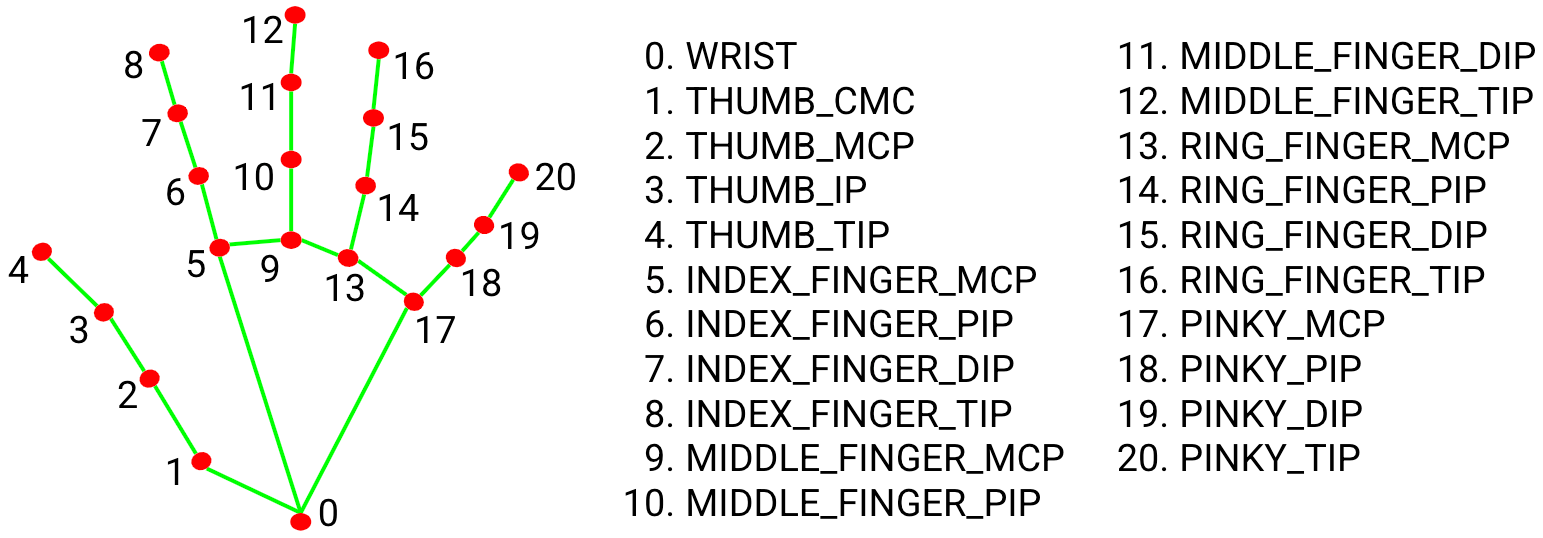
\includegraphics[width=\textwidth, keepaspectratio]{img/hand_landmarks.png}
  \caption{Landmarks extracted from detected hands by the MediaPipe hand solution.}
  \source{Adapted from \citetitle{mp-hands} \cite{mp-hands}.}
  \label{fig:hand-landmarks}
\end{figure}

The conversion from landmarks to gestures performed by the \texttt{gestures} has been designed as a simple but effective way to identify a limited set of hand positions without relying on complex machine-learning solutions. This conversion works by using the landmark coordinates to define two vectors per finger of the hand. One of the vectors points from the base of the hand (wrist landmark) to the base of each finger (points 1, 5, 9, 13, and 17 in Figure \ref{fig:hand-landmarks}), and the other vector points from the base of each finger to its tip (points 4, 8, 12, 16, and 20 in Figure \ref{fig:hand-landmarks}). With the vectors defined, the dot product vector operation is employed to calculate the relative angle of each finger with the base of the hand, as shown in Figure \ref{fig:vector-calcs}. Equations \ref{eq:vectors} and \ref{eq:angles} show example calculations for the index finger.

\begin{eqnarray}
    \vec{a} = P_5 - P_0\;\;\;\;\;\;\;\;\;\;\;\;\;\;\;\; \Vec{b} = P_8 - P_5
    \label{eq:vectors}\\
    \angle (\vec{a}, \vec{b}) = \arccos(\dfrac{\vec{a} \cdot \vec{b}}{\lvert\vec{a}\lvert \lvert\vec{b}\lvert})
    \label{eq:angles}
\end{eqnarray}
\begin{conditions}
\vec{a} &   vector for the index base \\
\vec{b} &   vector for the index finger \\
P_x     &   coordinates of landmark x according to Figure \ref{fig:hand-landmarks} \\
\end{conditions}

\begin{figure}
  \centering
  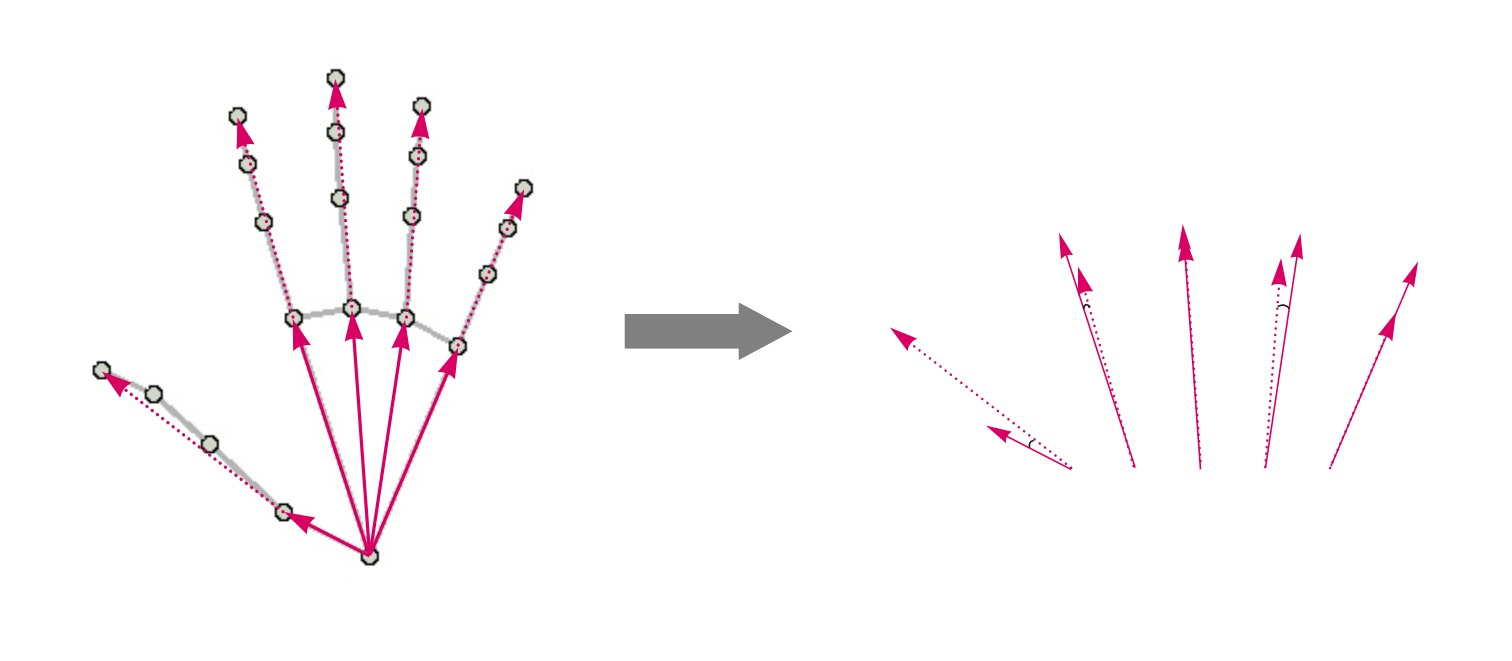
\includegraphics[width=0.9\textwidth, keepaspectratio]{img/hand-vectors.jpg}
  \caption{Vectors extracted from the detected features are used to calculate reference angles to determine hand gestures.}
  \label{fig:vector-calcs}
\end{figure}

By comparing the calculated angles to different thresholds, the module can determine whether each finger is extended or folded and in which direction it points. The thresholds have been determined experimentally by analyzing the angles calculated for the different fingers for different hand positions. Each possible gesture (see Figure \ref{fig:hand-gestures}) is then defined by the direction towards which each finger points, as detailed in the following list:
\begin{itemize}
    \item No hand: this happens when no landmarks can be extracted from the image. As a safety feature, the vehicle stops whichever previous commands it had in its queue and goes into Hold flight mode, hovering in the air while maintaining its position.
    \item Open hand: all five fingers extended, indicating a stop gesture. The drone holds at its current position.
    \item Fist: all five fingers folded into a fist. The drone arms and takes off if on the ground, or lands if already in the air.
    \item Backhand: the back of the hand is shown towards the camera, with the thumb pointing upwards and the other fingers pointing to the side. This gesture puts the drone in Return flight mode, where it climbs to a safe altitude and returns to the last takeoff position.
    \item Index finger pointing up: The index finger is extended and pointing roughly towards the top of the image (within $\pm$30 degrees). The drone enters Offboard flight mode, allowing direct velocity commands. The drone remains in this mode as long as the finger is extended, and its movement can be controlled with any of the next four commands.
    \item Index finger pointing to the right: The index finger points to the right of the image (between 30 and 90 degrees from the top). The drone rolls towards its right side at a speed of 1 m/s.
    \item Index finger pointing to the left: Same as above, but the index finger points to the left of the image. The drone rolls towards its left side.
    \item Thumb pointing to the right: The index finger is extended up (to maintain Offboard flight mode) while the thumb is folded over the palm, pointing towards the right of the screen. This gesture makes the drone pitch forward at a steady speed of 1 m/s.
    \item Thumb pointing to the left: Similar to the previous gesture, but the drone pitches backwards when the thumb points to the left of the screen.
\end{itemize}

\begin{figure}
  \centering
  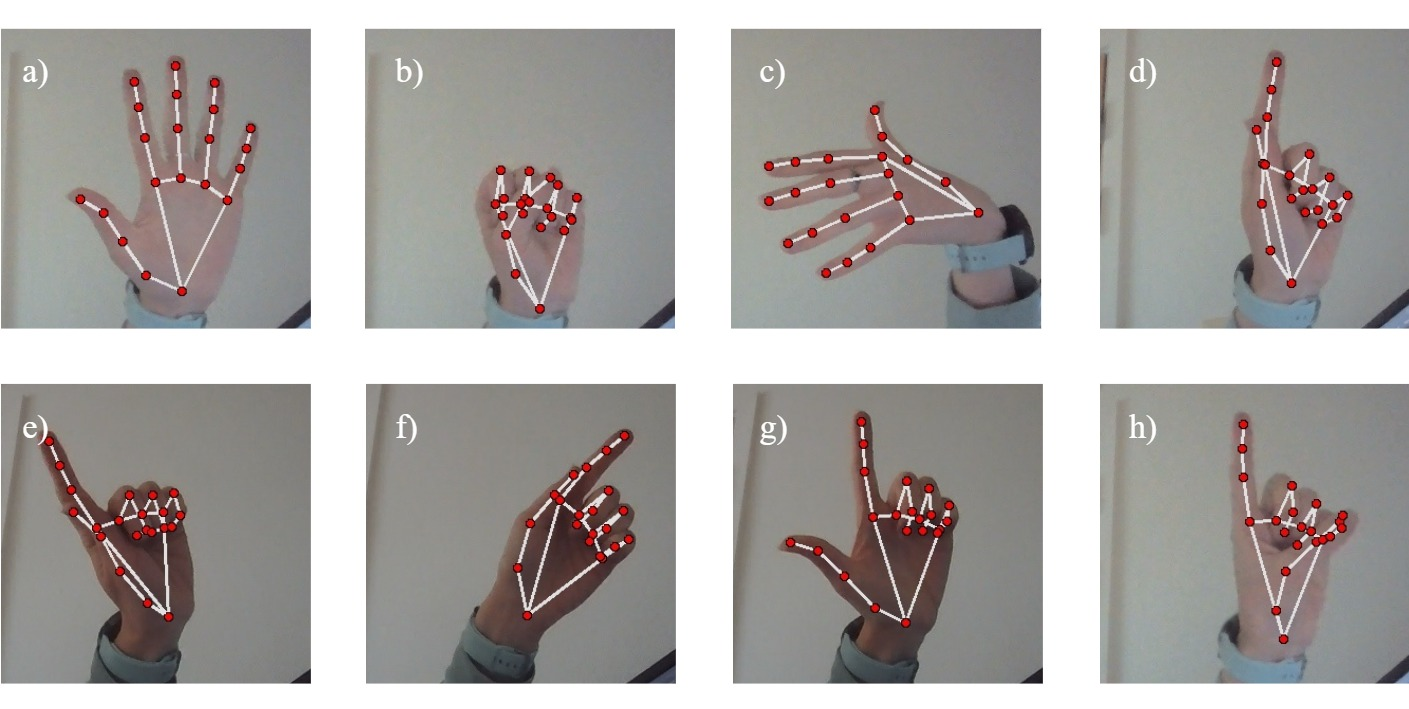
\includegraphics[width=\textwidth, keepaspectratio]{img/hand-gestures.jpg}
  \caption{Gestures detected by the program to control the drone's movement. a) Open hand, b) fist, c) backhand, d) index point up, e) index point left, f) index point right, g) thumb point left, h) thumb point right}
  \label{fig:hand-gestures}
\end{figure}


The program execution is outlined in Figure \ref{fig:hands-loop}.
After all the initial parameters have been set, a secondary thread is started to run the pilot queue detailed in \ref{subsec:pilot-module}, which waits for new commands to be added.
The main thread runs a GUI loop that continuously processes gestures calculated from retrieved images and generates actions that are queued for the pilot.
It also recognizes user input on the keyboard to control the vehicle directly, according to the mapping defined in the \texttt{input} module\footnote{\url{https://github.com/l-gonz/tfg-giaa-dronecontrol/blob/main/dronecontrol/common/input.py}}.


\begin{figure}
  \centering
  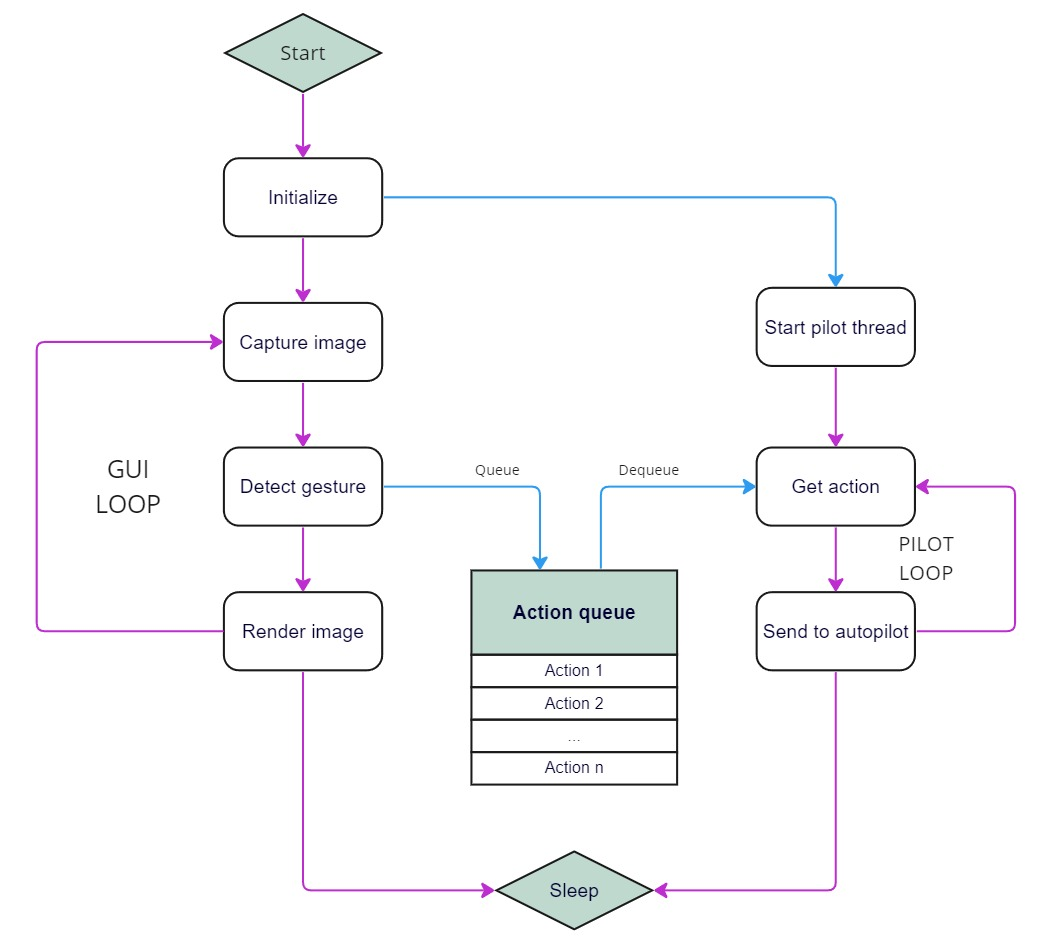
\includegraphics[width=0.8\textwidth, keepaspectratio]{img/hand-loop.jpg}
  \caption{Execution flow for the running loop in the hand-gesture control solution.}
  \label{fig:hands-loop}
\end{figure}

A complete run of this solution is detailed in Section \ref{subsec:fl-test-4}.
